\documentclass[12pt, aspectratio=43]{beamer}

%Tue font package
\usepackage[T1]{fontenc}

\usepackage{hyperref}

%Tue beamer theme
\usetheme[department=winuk, official=false, theme=darkblue, innovation=false]{tue2008}
\mode<presentation>

\title{Sharing Experience about Graduation Project}
\author{Tianyu Liu}
\date{May 24, 2018}


\begin{document}
    
    
%Title
\begin{titleframe}
\end{titleframe}

\begin{frame}{Table of Contents}
\begin{itemize}
    \setlength\itemsep{1em}
    \item Self-introduction
    \item Finding a graduation project
    \item Conducting a graduation project
    \item Practical information (esp. non-EU/EEA students)
\end{itemize}
\end{frame}

\begin{frame}{Introduction about Myself}
\begin{itemize}
    \setlength\itemsep{1em}
    \item At Philips Healthcare
    \item CSE - Software Science
    \item Software Engineering and Technology (SET) Group
    \item Project about code modernization
\end{itemize}
\end{frame}

\begin{frame}{Finding a Graduation Project}
Several criteria...
\end{frame}

\begin{frame}{Finding a Graduation Project}
\begin{center}
    
\includegraphics[scale=0.3]{images/Interests.png} \\
    INTERESTS
\end{center}
\end{frame}

\begin{frame}{Finding a Graduation Project}
\begin{center}
    
\includegraphics[scale=0.2]{images/WorkingEnvironment.png}
    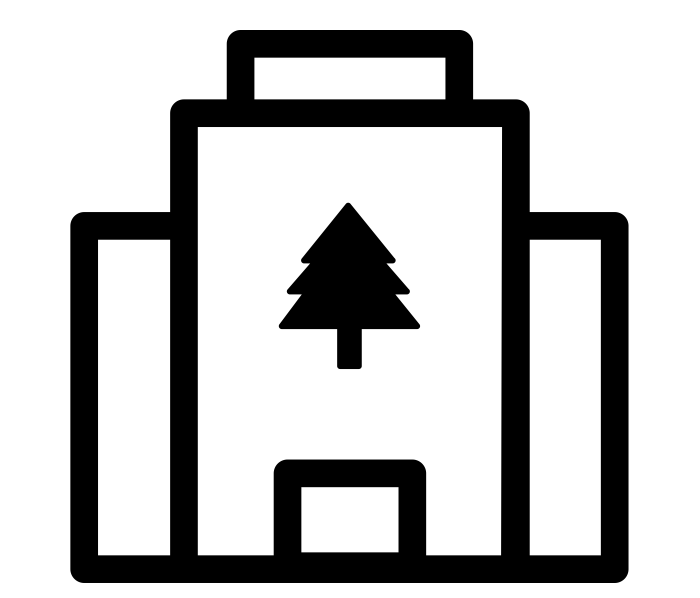
\includegraphics[scale=0.2]{images/OfficeEnvironment.png} \\
    WORKING ENVIRONMENT
\end{center}
\end{frame}

\begin{frame}{Tips and Tricks}
\begin{center}
    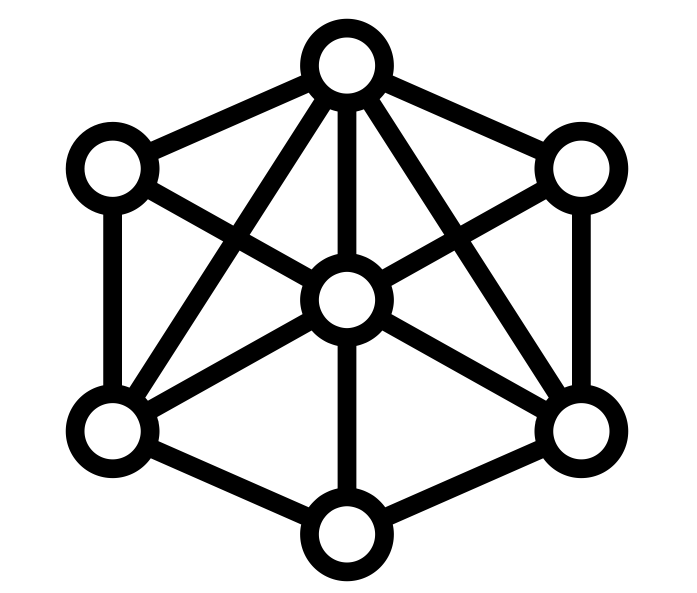
\includegraphics[scale=0.35]{images/Connection.png} \\
    CONNECTION
\end{center}
\end{frame}

\begin{frame}{Conducting a graduation project}

\includegraphics[scale=0.08]{images/Happy.png}
\begin{itemize}
    \item Experience to work in big company
    \item Meet new people, share life experiences
    \item Get allowances :)
\end{itemize}

\includegraphics[scale=0.08]{images/Sad.png}
\begin{itemize}
    \item Meetings, protocols, rules...
    \item Fruitless training and courses
    \item Lack of supervision and discussion
\end{itemize}

\end{frame}

\begin{frame}{Nuffic-Agreement}
\begin{center}
    
\includegraphics[scale=0.5]{images/NufficStd.png}
\end{center}
\end{frame}

\begin{frame}{Nuffic-Agreement}
\begin{center}
    
\includegraphics[scale=0.5]{images/NufficAnother.png}
\end{center}
\end{frame}

\begin{frame}{Practical information}
\begin{center}
    
\includegraphics[scale=0.25]{images/Paperwork.png} \\
    Paperworks
\end{center}
\begin{itemize}
    \item Nuffic agreement - ECTs, courses.
    \item Study program - make sure it is delivered safely.
    \item Insurance - avoid a fine. 
\end{itemize}
\end{frame}

\begin{frame}{Thanks!}
\begin{center}
    
\includegraphics[scale=0.17]{images/Question.png}
\end{center}
E-mail me if you have more question: \href{mailto:t.liu.1@student.tue.nl}{t.liu.1@student.tue.nl}
\bigbreak
You can also find this slide at:
\url{https://github.com/t-liu93/Start-graduation-project-meeting/releases/latest}
\end{frame}


\end{document}